% --
% test bench

\section{Test Bench of best Neural Network Architectures}\label{sec:exp_tb}
This section compares the best neural network architectures in terms of noise and shift invariance to fixed test wave files.
The test wave files are recorded by the author and its length is cut, so that by using a the fixed input frames of 500ms, both end positions consists at least of half of the wave file information.
Only the L5 labels were used.

\subsubsection{Shift invariances}
Shift invariances is very important for audio classification, e.g. the waveform should be still classified the same when shifted a little bit in time.
However the restricted frame size of 500ms makes this task very difficult, as it is already known that not all information can fit in there, e.g. like the \enquote{t} in \enquote{left} or \enquote{right} is often missed.
The figures in this section present a correct classification with a colored pixel and an incorrect with a white pixel.
The examples from the adversarial training section are shown in \rfig{exp_tb_shift_fc3}.
\begin{figure}[!ht]
  \centering
    \subfigure[adv init]{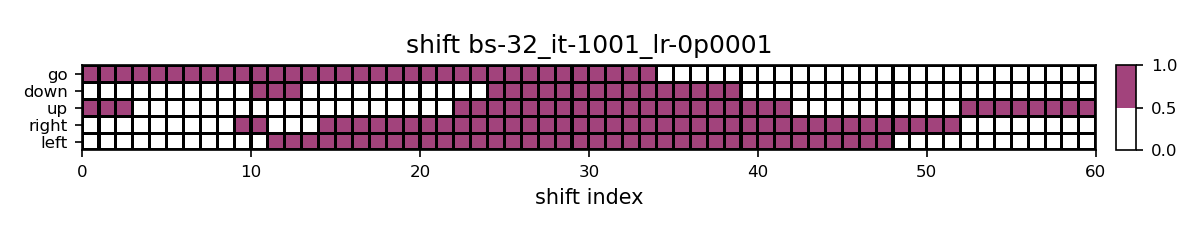
\includegraphics[width=0.45\textwidth]{./5_exp/figs/exp_tb_shift_fc3_adv}}
    \subfigure[random init]{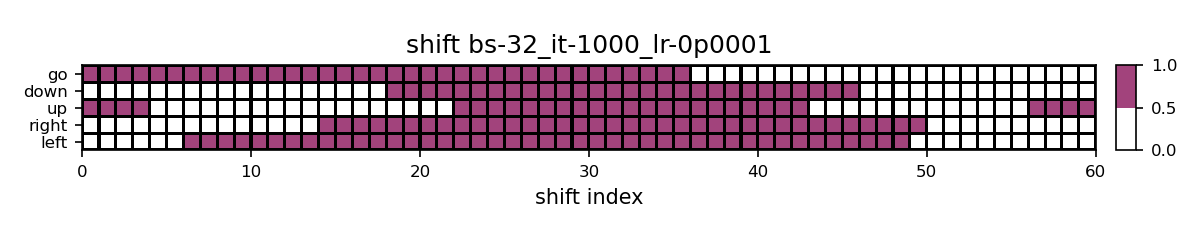
\includegraphics[width=0.45\textwidth]{./5_exp/figs/exp_tb_shift_fc3_random}}
  \caption{Shift invariance of L5-n500, c1d0dd0e0-norm1-it1000-bs32-lr0.0001-mo0.5 once with random init and once with adv init with dec-itl1000.}
  \label{fig:exp_tb_shift_fc3}
\end{figure}
\FloatBarrier
\noindent


\subsection{Noise invariances}
Noise invariance is a good trait in the classification of audio data.
That is because the usage of bad microphones or recording set ups may add a lot of noise to the audio and therefore might also disturb the classification accuracy a lot.
To create a test upon noise invariance, artificial normal noise is added to the test audio files.
In the plots this is indicated in the x-axis of the plots as SNR. 
A SNR level of zero means there is equal energy of noise and signal, therefore this is already pretty much disturbed.
in \rfig{exp_tb_noise_fc3} is the noise invariance from the example in the adversarial training section.

\begin{figure}[!ht]
  \centering
    \subfigure[adv init]{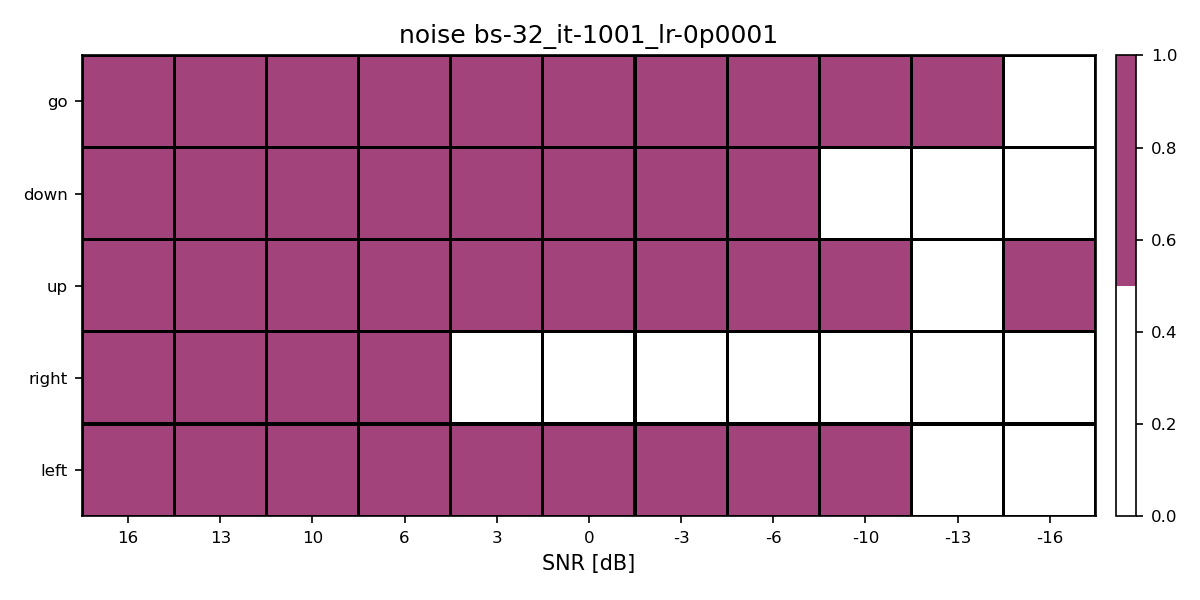
\includegraphics[width=0.40\textwidth]{./5_exp/figs/exp_tb_noise_fc3_adv}}
    \subfigure[random init]{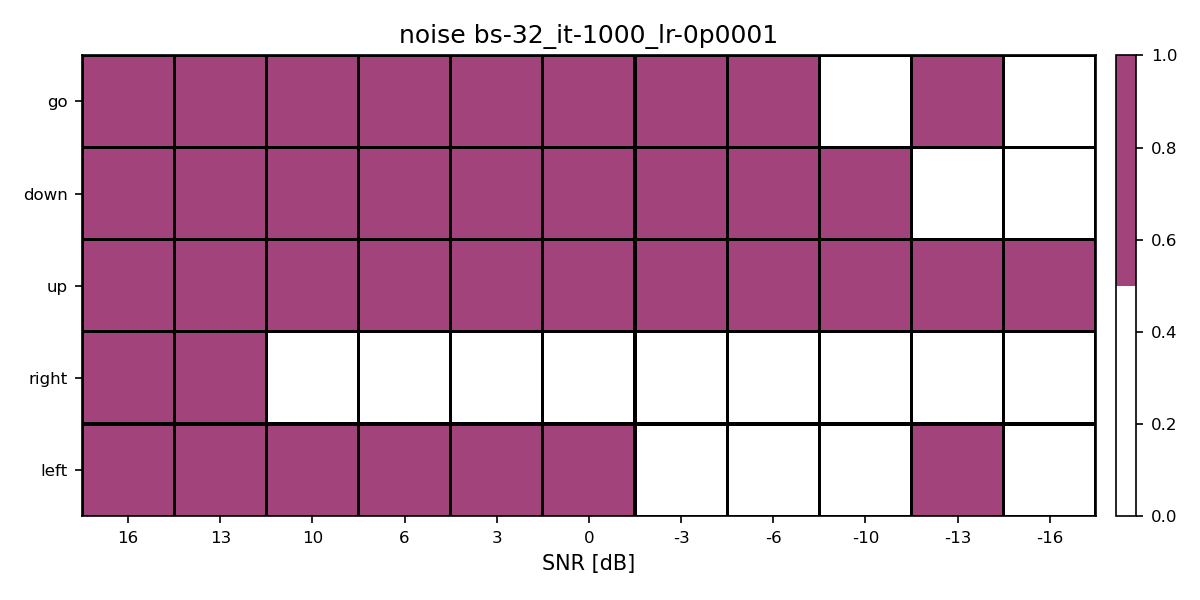
\includegraphics[width=0.40\textwidth]{./5_exp/figs/exp_tb_noise_fc3_random}}
  \caption{Noise invariance of L5-n500, c1d0dd0e0-norm1-it1000-bs32-lr0.0001-mo0.5 once with random init and once with adv init with dec-itl1000.}
  \label{fig:exp_tb_noise_fc3}
\end{figure}
\FloatBarrier
\noindent